\documentclass[english]{article}
 
\usepackage[utf8]{inputenc}
\usepackage[T1]{fontenc}
\usepackage{babel}
\usepackage{advdate}
\usepackage{graphicx} 
\usepackage{amsmath} 
\usepackage{algorithm}
\usepackage[noend]{algpseudocode}

\makeatletter
\def\BState{\State\hskip-\ALG@thistlm}
\makeatother


\begin{document}
\[\begin{titlepage}
\SetDate[30/01/2018]
\newcommand{\HRule}{\rule{\linewidth}{0.5mm}}
\center 
\textsc{\LARGE Universite Paris Dauphine}\\[1.5cm] 
\textsc{\Large Big Data}\\[0.5cm]
\HRule \\[0.4cm] { \huge \bfseries
Single-source shortest path - Djikstra Algorithm}\\[0.4cm] \HRule \\[1.5cm]
\begin{minipage}{0.4\textwidth}
	\begin{flushleft} \large
		\emph{Students}
		\\ Elie \textsc{Abi Hanna Daher}
		\\ Bilal \textsc{El Chami}
		\\ Badr \textsc{Erraji}
	\end{flushleft}
\end{minipage}
~
\begin{minipage}{0.4\textwidth}
	\begin{flushright} \large
		\emph{Professor} 
		\\ Mr Dario  \textsc{Colazzo}
		\\  \hspace{1cm}
		\\  \hspace{1cm}
	\end{flushright}
\end{minipage}\\[2cm]
{\large \today}\\[2cm]

\includegraphics[width=8cm]{img/dauphine.png}
\vfill
\end{titlepage}
 
\tableofcontents 
\newpage

\section{Project goal}
The goal of the project is to find the shortest paths from a source node to all other nodes in the graph using the Dijkstra’s algorithm. The algorithm should be implemented in both Python-Hadoop and Spark. \\

A long side the implementation, a scalability experiments is needed to check the performance of the algorithm implemented.

\section{Dijkstra Algorithm}
The Dijkstra’s algorithm finds the shortest path from source to all other nodes. The djikstra algorithm is very similar to the BFS algorithm, the only difference is that the distance between neighbors isn't 1, distance can differ from a neighbor to another.

Let's call the first node we begin with the \textbf{Start Node}, 
the distance of every other node is set relatively to the \textbf{Start Node}. Djikstra will allocate a certain value (the distance of the node to the \textbf{Start Node}) to every node ( by convention infinity) and then will try to correct them gradually as iterations take place.


\newpage

\section{Implementation}

\subsection{Input}

\subsubsection{Data}
The map task should receive the following information
\begin{itemize}
\item node
\item distance
\item neighbors data that contains the list of neighbors with their respective distance to the node
\item path
\end{itemize}
So let's take the following example with 1 being the start node :
\begin{figure}[h]
\centering
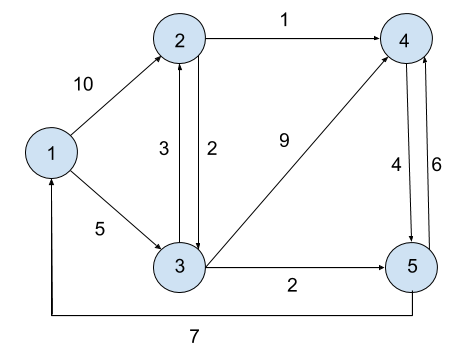
\includegraphics[width=8cm]{img/data-example.png}
\caption{Example of a graph}
\end{figure}
\\
For the first iteration, the path will be empty. So input data will look like this :
\begin{itemize}
\item 1 0 2,10:3,5:
\item 2 999 3,2:4,1:
\item 3 999 2,3:4,9:5,2: 
\item 4 999 5,4:
\item 5 999 1,7:4,6:
\end{itemize}
So as you can see, the start node has a distance of 0, and all other node have a distance of 999 which represent an infinite number. The neighbor list contains each neighbor node with their respective distance, the neighbors and the distance are separated by a "," and neighbors are separated by ":".

\subsubsection{Prepare}
Technically, the format we set for the data is very hard to implement to a large graph. Usually the graph is represented by the distance between nodes. So for the graph provided in the previous page, the input data will look like this 
\begin{itemize}
\item 1 2 10
\item 1 3 5
\item 2 3 2
\item 2 4 1
\item 3 2 3
\item 3 4 9
\item 3 5 2
\item 4 5 4
\item 5 1 7
\item 5 4 6
\end{itemize}
We created a job MapReduce - called prepare that will format the usual format of a graph to the format we are asking for.

\subsection{Mapper}
A map task receive (K,V)
\begin{itemize}
\item Key : node
\item Value : distance, neighbors data, path
\end{itemize}
In the first iteration, the path will be empty. \\
The map task will : 
\begin{enumerate}
\item emit the node with his information (distance, neighbors data and path)
\item  $\forall$ neighbor $\in$ neighbors, it will emit 
	\begin{itemize}
	\item Key : neighbor
	\item Value : (node distance + distance of node to the neighbor , node path + neighbor).
	\end{itemize}
\end{enumerate}

The pseudo code of the mapper is as follow : 
\begin{algorithm}[h]
\caption{Mapper}\label{mapper}
\begin{algorithmic}[1]
\Procedure{Map \emph{(node, (distance, neighbors, path))} }{}
\State \textbf{Emit} \emph{(node, (distance, neighbors, path))}
\State \textbf{for all} \emph{ neighbor $ \in$ neighbors } \textbf{do}
\State $\textit{ dist} \gets \textit{distance} + \textit{neighbor.distance} $
\State $ \textit{ p} \gets \textit{path} + \textit{neighbor.id} $
\State \textbf{ Emit} \emph{(neighbor.id, (dist, p))}
\EndProcedure
\end{algorithmic}
\end{algorithm}

\newpage
\subsection{Reducer}
The reduce will gather the possible distance for each node and selects the minimum one and set the path of the minimum one selected

\subsection{Job Chaining}
Since Dijkstra algorithm is iterative and we were using python streaming in for the project, we needed to execute several MapReduce steps with overall job scenarios, which means the last reduce output will be used as input for the next map job.
Map1 -> Reduce1 -> Map2 -> Reduce2 -> Map3...
So the simplest way to achieve it was by creating a shell script, that automates what we were doing manually.
The script launches the Hadoop streaming job, merges the output parts into one file and then moves it into the data directory so it can be used as input for the next job.
It’s not the optimal solution but it can do the job in an “acceptable” amount of time.

\section{Results}

\subsection{Hadoop}

\subsection{Spark}

\section{Performance}

\newpage

\begin{thebibliography}{9}
\bibitem{cloud-computing-lecture} \textit{Cloud Computing Lecture 4 - Graph Algorithms with MapReduce}. Jimmy Lin, The iSchool, University of Maryland, February 6, 2008.
\end{thebibliography}
\newpage
\appendix
\section{Appendix example}
This an example of appendix

\]
\end{document}